\documentclass{report}
\usepackage{amsmath}
\usepackage{graphicx}
\usepackage{hyperref}
\usepackage{rotating}

\hypersetup{colorlinks=true}
\hypersetup{urlcolor=blue}

\begin{document}

\begin{titlepage}
\centering

\includegraphics{images/cstart_logo} \\
\Large{\href{http://www.cstart.org}{Collaborative Space Travel and Research Team}} \\
\vspace{0.5cm}
\large{``Space exploration, by anyone, for everyone''} \\
\vspace{4.0cm}
\Large{CLLARE:} \\
\Large{Collaborative Lunar Landing and Research Expedition} \\
\Large{Project Overview} \\
\vspace{2.0cm}
\normalsize{Luke Maurits, \\
Add your name here, \\
If you contribute material, \\
Use alphabetical order} \\
\vspace{4.0cm}

\includegraphics{images/cc_badge} \\
This document is licensed under the \\
\href{http://creativecommons.org/licenses/by-sa/3.0/}{Creative Commons Attribution-Share Alike 3.0 license}
\end{titlepage}

\tableofcontents

\chapter{Introduction}

\section{What is CLLARE?}

The Collaborative Lunar Landing and Research Expedition (CLLARE) project is a proposed spaceflight project with the goal of landing a single human on the moon and returning them safely to Earth.  By using a reduced crew size, modern technology and a design philosophy emphasising simplicity and reusability, CLLARE endeavours to be an extremely low-cost project in comparison to Apollo or Constellation.

CLLARE is an ``open source'' spaceflight project.  What does this mean?  It means that documents such as this one and others which describe CLLARE in intimate technical detail, including spreadsheets and CAD files, are available for free under the Creative Commons Attribution Sharealike 3.0 license, so that anybody can copy, distribute and modify them.  It means that computer code to handle every aspect of planning and running CLLARE is available for free under the GNU General Public License 3,0, so that anybody can copy, distribute and modify it.  Anybody who has the desire, determination and money can build and launch the CLLARE hardware without any fear of legal issues (at least not from the people who planned CLLARE - some countries may have restrictions on who can launch what into space, when and where).  It means that anybody with the interest and knowledge can help refine the CLLARE project.

\section{Who is organizing CLLARE?}

CLLARE is a project of the Collaborative Space Travel and Research Team (CSTART).  CSTART is a non-government, non-profit space agency run by volunteers.  It provides online services to facilitate the planning and promotion of open source projects related to space travel and space research, like CLLARE.  It also attempts to raise the money required to fund these projects, or at least to fund the construction of proof--of--concept mock ups.  In the future CSTART may organize and fund space travel and research related prizes, with the condition that all entries are released under open source licenses at the end of the competition.

\section{How can I get involved in CLLARE?}

TODO: Expand on this!  See the page ``\href{http://cstart.org/wiki/Getting_involved_in_CLLARE}{Getting involved in CLLARE}'' of the CSTART Wiki.

\section{How can I suggest changes/corrections/improvements to this document?}

TODO: Expand on this!  Email Luke Maurits (\texttt{lmaurits -at- cstart -dot- org}).

%%%%%%%%%%%%%%%%%%%%%%%%%%%%%%%%%%%%%%%%%%%%%%%%%%

\chapter{Project Overview}

In this chapter we provide a high--level overview of the CLLARE project.  We discuss the flight plan for manned lunar landing flights, introduce the core hardware for carrying out such flights and the various possible configurations of this hardware, discuss launch options for getting the hardware configurations off the ground, and propose a program of flights gradually stepping from suborbital to lunar landing flights, effectively replicating the Mercury, Gemini and Apollo projects of early US manned spaceflight with a single set of hardware.  Later, in chapter \ref{chap:numeric} we present a numerical analysis of the project, estimating required velocity changed (``delta-v's''), vehicle masses, fuel requirements and cost estimates.  Chapter \ref{chap:detail} presents more detailed descriptions of the hardware as it is planned thus far.

\section{Flight Plan Overview} \label{sec:flightplan}

The CLLARE flight plan is of the Lunar Orbit Rendezvous (LOR) format.  Overall, the flight plan is very similar to that of the Apollo project and should be quite familiar to space enthusiasts.

A spacecraft composed of several connected modules, with a one person crew, is launched into a circular low Earth ``parking orbit'' (altitude approximately 200 km), using a multiple stage rocket booster.  Following successful completion of various checks and tests, a Trans Lunar Injection (TLI) burn is performed, taking the spacecraft out of LEO and putting it on a trajectory bound for the moon.  Once the spacecraft is sufficiently close to the moon, a Lunar Orbit Insertion (LOI) or ``lunar capture'' burn slows the spacecraft down to such a speed that it enters a circular low lunar orbit (altitude approximately 100 km).

Two possible trajectories from LEO to low lunar orbit are considered desirable choices for the flight.  The optimal choice is a so-called ``free return trajectory'', in which, if the LOI burn is ommitted, the influence of the moon's gravity serves simply to turn the spacecraft around roughly 180 degrees, allowing a ``free return'' to Earth.  Such trajectories are attractive from a safety perspective, allowing damaged spacecraft without the ability to change course themselves to still return home safely.  However, they require the spacecraft to have a comparatively high velocity during their approach to the moon, necessitating both a more powerful TLI and LOI burn, and hence more fuel.  An alternative trajectory, chosen to minimise the required TLI and LOI burns, could lower the flight's fuel requirements significantly and may be chosen if this is necessary to get the total launch mass for the flight below acceptable limits.  The travel time to the moon is roughly 3 days for a free return trajectory and roughly 5 days for a minimal fuel trajectory.

Once in low lunar orbit, the astronaut transfers via a ``spacewalk'' (EVA) from the main cabin of the spacecraft to a separate, detachable vehicle designed for travel to and from the lunar surface.  Descent is achieved through the use of a Descent Orbit Insertion (DOI) burn, which changes the landing vehicle's orbit from a circular orbit to a highly eccentric orbit with a minimum altitude of around 20 km (anything lower is unsafe due to high mountains on the moon's surface).  At this minimum altitude, a powered descent begins, culminating in a soft landing.  The main spacecraft remains in its original circular orbit during the entire descent process.

After landing, the astronaut exits the landing vehicle and engages in a few hours of lunar EVA.  The activities to be conducted during EVA if CSTART organises a CLLARE flight have not yet been planned, but will be done so to maximise the scientific value of the expedition, subject to restrictions on equipment and landing site imposed by practical considerations.  At the end of EVA, the landing vehicle returns the astronaut to the vicinity of the orbiting main spacecraft, whereupon the astronaut transfers back to the previously occupied cabin.

Once the lunar rendezvous has been completed, a Trans Earth Injection (TEI) or ``lunar escape'' burn accelerates the spacecraft to a sufficiently high speed to escape the moon's gravitational field, leaving it on a course bound for Earth.  Note that the landing vehicle is left behind in lunar orbit, so that there is less mass to carry back to Earth, saving on fuel.  The travel time to Earth is roughly XXX days. 

Upon arrival at Earth, a module of the main spacecraft designed to survive atmospheric reentry separates from the spacecraft, with the astronaut inside.  The remainder of the spacecraft is left to burn up in an uncontrolled reentry.  The reentry vehicle survives the reentry and lands either in the ocean or on land, and the astronaut awaits recovery.

\section{Core CLLARE Hardware}

The CLLARE project is based around a set of five hardware items, referred to as the core CLLARE hardware.  By combining items from the core hardware in appropriate configurations, a number of different mission types can be flown, ranging from suborbital flights up to lunar landings of the form described above.  This approach allows a gradual, cost-effective progression toward the ultimate lunar landing goal.

The sections below introduce the core hardware items.  Chapter \ref{chap:detail} contains more detailed descriptions of each hardware item and its subsystems.  Later in this chapter, Section \ref{sec:config} describes the various configurations of the hardware items which can be used to support a range of mission profiles.

\subsection{The CLLARE Command Module}

The \href{http://cstart.org/wiki/CLLARE_Command_Module}{CLLARE Command Module} (CM) is a one-person spacecraft in the ``truncated cone and cylindrical nose'' shape of the Mercury and Gemini spacecraft, which strongly influenced its design.  The CM contains sufficient onboard supplies of all required consumables to support its occupant for a duration of 24 hours, including support for one repressurisation of the capsule after extra vehicular activity (EVA) via an ingress-egress hatch.  An ablative heat shield permits the CM to reenter the Earth's atmosphere.  The CM will be capable of landing in water and possibly also on land.  Suggested landing options include parachute, paraglider and ballute.  The CM will be designed to be as reusable as possible.

The CM plays the role of the ``main cabin'' and ``reentry vehicle'' of the modular spacecraft described in Section \ref{sec:flightplan}.

\subsection{The CLLARE Orbital Support Module}

The \href{http://cstart.org/wiki/CLLARE_Orbital_Support_Module}{CLLARE Orbital Support Module} (OSM) is a small, truncated cone shaped module which attaches to the rear of the CLLARE CM.  The slope of the OSM is equal to the slope of the CM so that a mated CM-OSM combination has the appeareance of a single large truncated cone with a cylindrical nose.  The OSM facilitates the use of the CM for orbital flights in three ways:
\begin{enumerate}
\item The OSM contains a set of small retro rockets for providing deorbit burns.  These are simple solid or hybrid rockets designed for single use.  The retro rocket assembly is designed in such a way that it can be completely removed when the OSM is used as part of a hardware configuration where the assembly is unecessary.
\item The OSM contains a set of additional RCS thrusters.  These thrusters can work together with the CM's RCS thrusters (which alone provide only attitude control) to allow accurate orbital maneuvering, including translation.
\item The OSM can optionally contain supplies of various consumables to supplement those stored onboard the CM, extending its endurance from 24 hour to at least 7 days.
\end{enumerate}
The OSM is not equipped to survive reentry.  It is separated from the CM immediately after the deorbit burn and burns up in the atmosphere.

\subsection{The CLLARE Propulsion Module}

The \href{http://cstart.org/wiki/CLLARE_Propulsion_Module}{CLLARE Propulsion Module} (PM) attaches to the rear of a CLLARE Orbital Support Module.  The module contains a large propellant tank and a symmetric arrangement of liquid bipropellant rockets at its end.  The PM is able to provide large changes in velocity to a CM-OSM combination, allowing high-altitude orbital flights or circumlunar flights.  The PM can also be used to perform deorbit burns, replacing the Retro Module for flights using a PM.  The PM is not equipped to survive reentry and burns up along with any other modules.

Two variants of the PM are proposed, a ``light'' variant (PML) and a ``heavy'' variant (PMH).  The variants differ only in the length of their tanks (and hence the amount of delta-v they can impart). The PML is intended for use in circumlunar flights, whereas the PMH is intended for lunar landing flights.

\subsection{The CLLARE Lunar Lander}

The \href{http://cstart.org/wiki/CLLARE_Lunar_Lander}{CLLARE Lunar Lander} (LL) is a light weight, open cabin lunar landing craft.  Unlike the Apollo lunar lander (and like the planned Soviet lunar lander), the LL is not composed of two separable stages.  The entire structure undergoes a lunar descent and a lunar ascent, with the same engine and set of fuel tanks used for both directions.  The lunar lander's engine is a liquid bipropellant rocket and is the same engine as used in the CLLARE Propulsion Module's symmetric arrangement, meaning only one liquid rocket engine is used anywhere in the core hardware.

The LL plays the role of the ``landing vehicle'' of the modular spacecraft described in Section \ref{sec:flightplan}.

\subsection{The CLLARE Lunar EVA Suit}

The \href{http://cstart.org/wiki/CLLARE_Lunar_EVA_Suit}{CLLARE Lunar EVA Suit} is a space suit suitable for use with EVA in LEO, lunar orbit and on the lunar surface.  (WE NEED TO EXPAND ON THIS)

\section{Core Hardware Configurations} \label{sec:config}

The CLLARE core hardware has been designed in such a way as to facilitate a range of configurations fulfilling a range of flight types.  The following subsections describe these configurations.  Figure \ref{fig:configs} shows diagrammatic representations of the different configurations.

\begin{figure}[h] \label{fig:configs}
\centering
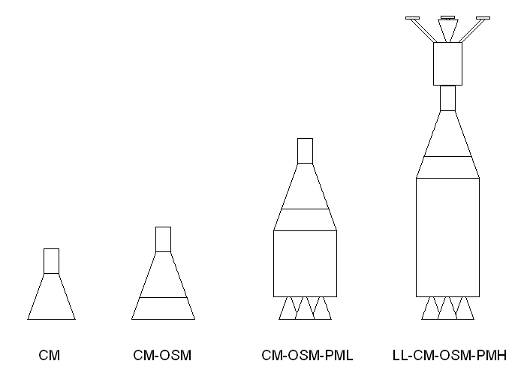
\includegraphics[scale=0.6]{images/cllare_hardware_configs}
\caption{Various configurations of the CLLARE core hardware.  From left to right: suborbital, low altitude orbital, high altitude orbital or circumlunar, and lunar landing.  Diagrams not to scale.}
\end{figure}

\subsection{Suborbital configuration}

The simplest configuration of the core hardware is that consisting of the CM alone.  This configuration is appropriate only for suborbital space flights (in which the CM is boosted in a mostly vertical trajectory to an altitude of greater than 100km, but does not obtain the required tangential velocity for orbit).  Such flights last for approximately 15 minutes and so the CM's 24 hours worth of onboard consumables are more than adequate.
 
This configuration is functionally equivalent to the US Mercury craft, when it was used for suborbital flights early in proejct Mercury.

\subsection{Low apogee orbital configuration}

The simplest non--trivial configuration of the core hardware consists of a CM coupled to an OSM (denoted CM-OSM).  This configuration is appropriate for orbital flights where the orbit is low enough that the configuration can be inserted directly into it by the launch vehicle (e.g. around 200 km altitude).

There are two variants of this configuration: for short duration orbital flights (lasting less than 24 hours total), the CM's onboard consumables are sufficient and the OSM need not have its consumables tanks attached.  For long duration orbital flights (lasting greater than 24 hours), the OSM must be equipped with consumable tanks to supplement the CM's onboard consumables.  The OSM must have its retro rockets equipped in both configurations to provide deorbit capability.

This hardware configuration is functionally equivalent to Mercury when it was used for orbital flights later in project Mercury or, if EVA is performed during orbit, to the US Gemini craft.

\subsection{High apogee orbital and circumlunar configuration}

The second most complicated configuration of the core hardware consists of a CM coupled to an OSM which is in turn coupled to a ``light'' PM (denoted CM-OSM-PML), with consumables but no retro rockets in OSM.  This configuration is appropriate both for orbital flights where the altitude is sufficiently high that the spacecraft must use its own propulsion capabilities to be lifted into to the orbit after being inserted into a lower orbit by the launch vehicle, and circumlunar flights, where a TLI burn puts the craft on a free--return rajectory, passing around the moon without the need for further significant propulsion.  In both of these cases, the PML is used to provide the necessary velocity changes.  The OSM does not have its retro rockets equipped in this configuration as the PML is also able to provide deorbit capability.

This configuration is functionally equivalent to both a Gemini capsule docked with an Agena Training Vehicle booster, and an Apollo Command Module and Service Module (CSM) combination (with no docked Lunar Module) - the OSM-PML combination is roughly functionally equivalent to the the Apollo SM.

\subsection{Lunar landing configuration}

The final and ``ultimate'' configuration of the core hardware consists of a CM-OSM-PMH configuration (like the previous configuration but with the heavy variant of the PM), with a Lunar Lander attached to the nose of the CM (denoted LL-CM-OSM-PMH).  This configuration is suitable for lunar landing flights.

In this configuration, the PMH provides the propulsion required for TLI, LOI and TEI burns.  Transfer from the CM to the LL in lunar orbit is achieved via a short EVA.  Note that, unlike Apollo, the LL is attached to the nose of the CM from the beginning, rather than having to be transferred there from behind after TLI.  This is made possible by the use of an aerodynamic fairing on the planned launch vehicle (see Section \ref{sec:launchopt} later in this chapter).

It is noteworthy that in this configuration, should the PMH be damaged during a flight, the LL engine can provide emergency propulsion for a LL-CM-OSM ``subcraft'' which separates from the PMH.  This technique would be very similar to that used on the infamous Apollo 13 flight.  We show later in Chapter \ref{chap:numeric} that a fully fuelled LL would be able to impart sufficient delta-v to a LL-CM-OSM subcraft for TEI from lunar orbit.

This configuration is functionally equivalent to the complete Apollo spacecraft, consisting of the CSM combination with the Lunar Module docked to the nose of the CM.

\section{Launch Options} \label{sec:launchopt}

In this section we discuss launch options for the various hardware configurations.  In order to do so we require estimates of the total masses of each of the configurations in ready--to--launch condition.  We do not justify the mass figures used for the discussion of launch options here -- the figures we use are derived in detail in Chapter \ref{chap:numeric}.

\subsection{Suborbital and low apogee orbital flights}

The proposed suborbital and orbital flight configurations (CM and CM-OSM) have estimated total masses in the vicinity of 1,000 kg and 1,250 kg, respectively.

CSTART is not aware of any man--rated commercial launch vehicles designed to carry payloads of this mass, so is considering the development of its own launch capabilities for these missions.  The current plan of approach is to use variably sized clusters of small, simple and inexpensive rockets to lift payloads around 1,000 kg in mass into LEO, a concept pioneered by the \href{http://en.wikipedia.org/wiki/OTRAG}{OTRAG company} project in the 1970s.  We are keen to use hybrid rocket engines for the small rockets due to their high levels of safety and excellent trade-off between simplicity and performance.

A group called \href{http://www.copenhagensuborbitals.com/}{Copenhagen Suborbitals}, based in Denmark, are currently working on a hybrid rocket engine designed to perform suborbital flights for a manned, lightweight ``micro space capsule''.  Copenhagen Suborbitals are already at the stage of performing static test firings of their rockets, with a first launch planned for mid 2010.  Like CSTART, Copenhagen Suborbitals is a volunteer operation funded by donations and sponsorships, with a strong commitment to open source principles.  The two groups are on friendly terms and CSTART hopes to gain valuable insight and experience from the Copenhagen Suborbitals team in constructing its own hybrid rocket launch systems.

\subsection{High apogee orbital and circumlunar missions}

The proposed high apogee orbital and circumlunar flight configuration (CM-OSM-PML) has an estimated total mass of 3679 kg, depending upon choice of propellant.

The \href{http://en.wikipedia.org/wiki/Soyuz-FG}{Soyuz-FG} is a man--rated launch vehicle with an extremely well established reliability.  It is used by the Russian Federal Space Agency (RKA) to transfer crews to the International Space Station in Soyuz spacecraft, which have a launch mass of around 7,000 kg.  It may be suitable for launching CM-OSM-PML configurations, subject to cooperation from the RKA.  A commercial version of this launch vehicle, the Soyuz-FG/Frigat, has a LEO payload of 7800 kg.  Commercial Soyuz-FG/Frigat launches are handled by the \href{http://www.starsem.com}{Starsem} company.  A total of 9 commercial launches have been carried out to date, although none have been manned.

\subsection{Lunar landing missions}

The proposed lunar landing configurations (LL-CM-OSM-PMH) has an estimated total masses in the vicinity of 10,000 kg, using liquid oxygen and liquid hydrogen as propellants.

The \href{http://spacex.com}{SpaceX} company's \href{http://spacex.com/falcon9.php}{Falcon 9} is a man-rated, two-stage booster capable of lifting 10,450 kg of payload into LEO.  The Falcon 9 is currently under development, but is nearly ready and may be suitable for launching lunar landing configurations of the CLLARE hardware.

The Falcon 9 is a strongly preferred launch option for lunar landing configurations, as its aerodynamic fairing facilitates positioning the LL infront of the CM from the beginning of the flight.  Without this fairing the LL would need to be stored behind the CM, necessitating either a docking operation after launch or a longer and more complicated transfer EVA.

\section{A proposed program of flights}

In this section we propose a program of 11 flights of the CLLARE core hardware, ranging through all the hardware configurations, with each item of core hardware testing in an unmanned capacity before a manned capacity.  The program culminates with a manned lunar landing by CLLARE 11, an ``accidental homage'' to mankind's first lunar landing Apollo 11.

CLLARE 1: Unmanned suborbital flight (closely monitored crash test dummy in CM, full telemetry reporting)

CLLARE 2: Manned suborbital flight

CLLARE 3: Unmanned orbital flight (closely monitored crash test dummy in CM, full telemetry reporting)

CLLARE 4: Manned orbital flight, no EVA

CLLARE 5: Manned orbital flight, including EVA

CLLARE 6: Unmanned high altitude orbital flight (to test PM)

CLLARE 7: Manned high altitude orbital flight, including EVA

CLLARE 8: Unmanned circumlunar flight (to test accuracy of free-return trajectory insertion)

CLLARE 9: Manned circumlunar flight

CLLARE 10: Manned flight into lunar orbital with unmanned landing (to test LL)

CLLARE 11: Manned lunar landing flight

%%%%%%%%%%%%%%%%%%%%%%%%%%%%%%%%%%%%%%%%%%%%%%%%%%

\chapter{Numerical Analysis} \label{chap:numeric}

In this chapter we present estimates, principled arguments and calculations to estimate the total mass and cost of flying various configurations of the CLLARE core hardware.  We conclude that a complete lunar landing mission based on the CLLARE hardware should cost no more than US\$50,000,000.

\section{Astrodynamics}

\subsection{Trans Lunar Injection burn} \label{sec:tli}

The speed of a spacecraft in a circular orbit $a$ m above a uniform spherical planet of radius $r$ m and mass $m$ kg is given by:
\begin{equation} \label{eq:v_orbit}
|v_{orbit}| = \sqrt{\frac{Gm}{a+r}},
\end{equation}
where $G = 6.67428 \times 10^{-11} m^3 kg^{-1} s^{-2}$ is the universal gravitational constant.

Earth has a mass of $m = 5.9736 \times 10^{24}$ kg and a mean radius of $r = 6,371,000$ m, so a spacecraft in a LEO of altitude $a = 200,000$ m has speed approximately $|v_{orbit}| \simeq 7910$ m/s.

The escape ``velocity'' (actually an escape speed, as direction is unimportant) at a point $a$ m above the surface of a uniform spherical planet of radis $r$ m is given by:
\begin{equation} \label{eq:v_escape}
|v_{escape}| = \sqrt{\frac{2Gm}{a+r}}.
\end{equation}
Using appropriate values for Earth, the escape speed is approximately $|v_{escape}| \simeq 11187$ m/s.

Thus the theoretically required delta-v for a TLI burn is:
\begin{equation}
|v_{escape}| - |v_{orbit}| \simeq 3276 m/s.
\end{equation}

Note that this figure is, in fact, an upper bound on the TLI delta-v.  It is possible to send a spacecraft from LEO to the moon without technically escaping Earth's gravity, by putting the space craft into a highly eccentric Earth orbit whose apogee is equal to or greater than the moon's distance from the Earth.  In practice, CSTART expects to use such an orbit to save on propellant mass, however for preliminary planning purposes we use the figure above.

\subsection{Lunar Orbit Insertion burn}

The delta-v required for Lunar Orbit Insertion depends upon the velocity of the spacecraft at the time it reaches a suitable distance from the moon for insertion; this velocity, in turn, depends on the TLI delta-v which was used.  For preliminary planning purposes, we use a required delta-v of 1000 m/s, which is an approximate figure for LOI on a free--return trajectory.  These trajectories involve the highest lunar approach delta-v of all trajectories which CSTART expects to consider.

\subsection{Trans Earth Injection burn}

The analysis for this burn's delta-v requirement is identical to that presented in section \ref{sec:tli}.  We use equations \ref{eq:v_orbit} and \ref{eq:v_escape} with appropriate lunar orbit values ($a = 100,000$ m, $r = 1,737,100$ m and $m = 7.3477 \times 10^{22}$ kg to find $|v_{orbit}| \simeq 1680$ m/s and $|v_{escape}| \simeq 2376$ m/s.

Thus the theoretically required delta-v for a TEI burn is:
\begin{equation}
|v_{escape}| - |v_{orbit}| \simeq = 696 m/s.
\end{equation}

\subsection{Lunar descent and ascent}

Determining the delta-v required for lunar descent and ascent is less straightforward than requiring the other delta-v figures.  We showed in the previous section that the orbital velocity for a 100 km lunar orbit is roughly 1860 m/s.  Since the LL is at rest after landing, descent and ascent both involve a literal change in velocity of that amount, for a total of 3720 m/s.  However, the requirement that the LL impact the moon's surface with both horizontal and vertical velocities as close to zero as possible prevents a straightforward application of exactly 1860 m/s of delta-v for descent, and similarly the need for the orbital velocity of 1860 m/s to be achieved at a particular hight and in a particular direction prevents a straightforward application of exactly 1860 m/s of delta-v for ascent.

The precise delta-v budget required for descent and ascent depends upon the particular descent and ascent strategies used.  These have not yet been planned for CLLARE (although when they are planned it seems likely that they will be planned so as to minimise total delta-v).

For the purposes of preliminary planning, we use a total descent and ascent delta-v requirement of 4700 m/s, based on the corresponding delta-v for the Apollo lunar landings.

\section{Mass figures}

\subsection{Consumables masses}

\subsubsection{Breathing gas}

There are two stores of oxygen involved in the CLLARE hardware: a store in the CM sufficient to support 24 hours of habitation, including $x$ EVAs (complete repressurisations of the cabin), and a store in the OSM, to support an addition 6 days of habitation, including an additional $y$ EVAs.

The two figures we require to estimate the required masses of oxygen for these two stores are an average oxygen consumption rate and a cabin oxygen capacity (assuming a 20\% oxygen atmosphere).

Various sources around the web suggest that the average adult human consumes around 550 L of oxygen per day.  Gaseous oxygen at typical Earth surface pressures has a density of about 1.4 g/L, so that the oxygen consumption rate is 770 g per day. 

The Mercury spacecraft had a habitable volume of 1.7 cubic metres.  We shall work with a slightly increased figure of 2.0 cubic metres, or 2000 L, to allow extra room for donning and removing an EVA suit.  To simplify calculations, let us work with a pressure of 1 atm (101.325 kPa) -- it will be easy to adjust our results for alternate pressures later.  Let us assume a cabin temperature of $20^\circ$ C.  Under these conditions, the \href{http://en.wikipedia.org/wiki/Ideal_gas_law}{ideal gas law} gives the cabin as containing 83.14 mol of gas.  If 20\% of this gas is oxygen, there are 16.63 mol of oxygen.  Diatomic oxygen has a molar mass of 32 g/mol, so this is 532 g of oxygen.

The remaining 80\% of the atmosphere must be composed of an inert ``filler gas'', and some of this gas must be stored for repressurisation after EVA.  Nitrogen is the most likely choice, to closely reproduce the atmosphere on Earth.  From our calcultions above, the pressurised cabin will contain 83.14 mol of gas.  If 80\% of this gas is nitrogen, there are 66.52 mol of nitrogen.  Diatomic nitrogen has a molar mass of 28 g/mol, so this is 1862.56 g or around 1.9 kg of nitrogen.

\subsubsection{Water}

20 L of water will provide 2 L per day for 10 days (longer than expected mission time), for a total mass of 20 kg.

\subsubsection{Methanol}

\subsection{Hardware masses}

\subsubsection{Command Module}

We derive an estimated mass for the empty CM vehicle by considering the masses of two similar existing spacecraft from the US manned spaceflight program, Mercury and Gemini.

The Mercury spacecraft is arguably the spacecraft most similar to the CLLARE CM, in that it is the only craft shaped like a truncated cone with a cylindrical nose which has a crew capacity of one.  However, the capabilities of the CLLARE CM exceed those of Mercury somewhat, in that the CLLARE CM supports EVA.  Since the CLLARE CM will require the addition of an ingress-egress hatch and also extra room in the crew cabin to facilitate the application and removal of a spacesuit, we expect the CLLARE CM to be slightly larger than Mercury.  Thus, a mass estimate derived from the mass of Mercury can be expected to be an \emph{underestimate} of the mass of the CLLARE CM.

Table \ref{tab:mercurymass} gives the masses of all the Mercury spacecraft subsystems (data taken from \href{http://www.astronautix.com/craft/mercury.htm}{Encyclopedia Astronautix}).  Beside each Mercury mass figure is an estimate of the mass of a corresponding CLLARE CM subsystem, with a justification.  This process leads to a total mass estimate of 932 kg.
 
\begin{sidewaystable}
\centering
\begin{tabular}{|l|c|c|l|}
\hline
Item	& Mercury mass & Est. CLLARE mass & Justification \\
\hline \hline
Structure		& 340 kg	& 340 kg & \\
Heat shield		& 272 kg	& 272 kg & \\
RCS			& 40 kg		& 40 kg & \\
Recovery equipment	& 60 kg		& 60 kg & \\
Navigation equipment	& 40 kg		& 10 kg & Crossbow make a GPS/IMU unit with mass 1.6 kg \\
Telemetry equipment	& 50 kg		& 10 kg & This is just some sensors and a single computer board \\
Electrical equipment	& 80 kg		& 10 kg & Ultracell XX55 has mass 1.6 kg \\
Communications system	& 20 kg		& 20 kg & \\
Crew seats and provisions & 80 kg	& 80 kg & \\
Environmental control system	& 50 kg		& 50 kg & \\
\hline \hline
\textbf{Total}	& 1032 kg & 892 kg	& \\
\hline
\end{tabular}
\caption{Mercury derived mass estimate}
\label{tab:mercurymass}
\end{sidewaystable} 

The Gemini spacecraft is the spacecraft with the most similar capabilities to the CLLARE CM, in that it allows EVA and can be adapted for long duration flights by the attachment of a supply module.  However, whereas the CLLARE CM has a crew of one, Gemini supported a crew of 2 (hence the name ``Gemini'' -- ``twins'').  It is fair to call the CLLARE CM a ``one--man Gemini''.  Thus, a mass estimate derived from the mass of Gemini can be expected to be an \emph{overestimate} of the mass of the CLLARE CM.

Table \ref{tab:geminimass} gives the masses of all the Gemini spacecraft subsystems (data taken from \href{http://www.astronautix.com/craft/gemini.htm}{Encyclopedia Astronautix}).  Beside each Gemini mass figure is an estimate of the mass of a corresponding CLLARE CM subsystem, with a justification.  This process leads to a total mass estimate of 1297 kg.

\begin{sidewaystable}
\centering
\begin{tabular}{|l|c|c|l|}
\hline
Item	& Gemini mass & Est. CLLARE mass & Justification \\
\hline \hline
Structure		& 638 kg	& 638 kg &  \\
Heat shield		& 144 kg	& 144 kg & \\
RCS			& 133 kg	& 133 kg & \\
Recovery equipment	& 98 kg		& 98 kg & \\
Navigation equipment	& 62 kg		& 10 kg & Crossbow make a GPS/IMU unit with mass 1.6 kg \\
Telemetry equipment	& 51 kg		& 10 kg & This is just some sensors and a single computer board \\
Electrical equipment	& 125 kg	& 10 kg & Ultracell XX55 has mass 1.6 kg \\
Communications system	& 26 kg		& 26 kg & \\
Crew seats and provisions & 426 kg	& 80 kg & Using figure from Mercury -- Gemini had two \\
				& 	&	& ejection seats (with rockets, parachutes, etc.) \\
Environmental control system	&  117 kg		& 117 kg & \\
\hline \hline
\textbf{Total}	& 1707 kg & 1123 kg	& \\
\hline
\end{tabular}
\caption{Gemini derived mass estimate}
\label{tab:geminimass}
\end{sidewaystable} 

Averaging our Mercury--derived underestimate of 892 kg and our Gemini--derived overestimate of 1123 kg, we estimate the empty mass of the CLLARE CM to be approximately 1008 kg.

\subsubsection{Orbital Support Module}

Mercury's retro rocket pack: 237 kg (seems awfully heavy)

Structural mass of Gemini's equipment module (much larger than our OSM): 250 kg

\subsubsection{Propulsion Module}

Estimating the mass of the PM is somewhat difficult.  A considerable proportion of the PM's total mass is contributed by its fuel tank.  The size of the tank, and hence its mass, depends on the total quantity of propellants required.  This, in turn, depends on the total mass of the hardware configuration, including the mass of the tank.

For a rough estimate, we consider masses of the \href{http://en.wikipedia.org/wiki/Space_Shuttle_external_tank}{Space Shuttle external tank}, which holds liquid oxygen and liquid hydrogen in cylindrical structure.  An estimate derived from a liquid hydrogen tank will represent a ``worst case'' estimate, since liquid hydrogen has an extremely low density and hence tanks to significant quantities of it must be large.

Let us consider the case where the entire hardware configuration for a lunar landing mission, with the Lunar Lander fuelled but the PM unfuelled has a mass of 4250 kg (this figure is based on considerable overestimates of the mass of other core hardware components).  To apply a total delta-v of $3276 + 1000 + 696 \simeq 5000$ m/s to this mass (for TLI, LOI and TEI) using a liquid oxygen and liquid hyrdogen engine with a specific impulse of 425 s would require approximately 9,200 kg of propellant (this calculation is made using the Tsiolkovsky rocket equation, which is introduced in Section \ref{sec:rocket_eq}).  This is about 1.3\% of the propellant capacity of the Shuttle's external tank.  If we use the approximation that a tank's mass is directly proportional to its capacity, we can estimate the mass of the PM's tank at 1.3\% of the Shuttle external tank.

There are a range of different models of external tank with differing masses.  The heaviest is the 35,000 kg Standard Weight tank and the lightest is the 26,500 kg Super Lightweight tank.  Using an average mass of 30,750 kg, our 1.3\% tank may have a mass in the vicinity of 385 kg.

Accounting for the extra mass of the PM's engines, supporting structures, etc., it seems like a total mass of 500 kg for an empty PM is a reasonable rough estimate.  This is for the PMH variant.  The PML variant has to impart roughly 60\% the delta-v of the PMH and so will be less massive.

\subsubsection{Lunar Lander}

For the purposes of initial considerations, we use an estimated mass of 300 kg for the unfuelled lunar lander. (TODO: Justify this -- there are some rough estimates in the forums that do so)

\subsection{Propellant masses} \label{sec:rocket_eq}

In this section we use the \href{http://en.wikipedia.org/wiki/Tsiolkovsky_rocket_equation}{Tsiolkovsky rocket equation} to estimate the required fuel masses for the mission, considering various fuel options.

The Tsiolkovsky rocket equation (hereafter ``the rocket equation'') relates the mass of an object, $m_0$, a desired delta-v for that object, $\Delta v$, the specific impulse of a propellant (in seconds), $I_{sp}$ and the mass $m_1$ of the object plus the quantity of propellant required to achieve the delta-v:
\begin{equation}
m_1 = m_0\exp \left( \frac{\Delta v}{9.8 I_{sp}} \right)
\end{equation}

\subsubsection{Propellant options}

The most likely propellants for use on CLLARE are considered to be liquid oxygen (LOX) oxidiser and liquid hydrogen (LH2) fuel, and LOX oxidiser and liquid methane (LCH4) fuel.

LOX/LH2 offers the greatest specific impulse, in the 400s--450s range.  However hydrogen has a very low density (leading to large, heavy storage tanks) and is highly explosive.

LOX/LCH4 offers a lower specific impulse than LOX/LH2, in the 350s--380s range, but methane is much denser than hydrogen and also safer.

\subsubsection{Circumlunar flights}

An ideal circumlunar flight of the CM-OSM-PML configuration, using a free-return trajectory, requires only a single burn: the TLI burn, which we found in \ref{sec:tli} to require a delta-v of 3276 m/s.  This delta-v must be applied to the mass of the CM-OSM-PML, which is estimaged at around 1750 kg.  For the lowest likely specific impulse of 300 s, the rocket equation gives a total fuelled mass of 5333 kg, and for the highest likely specific impulse of 450 s, the rocket equation gives a total fuelled mass of 3679 kg.

\subsubsection{Lunar landing flights}

Computing the propellant mass requirements for a lunar landing flight must be done in three steps.  We must compute the propellant mass required to carry the Lunar Lander to the lunar suface and back; We must compute the mass required to apply the TEI burn to the CM-OSM-PMH configuration; Finally, we must compute the mass required to apply the TLI burn to the CM-OSM-PMH configuration and the lunar lander, including the propellant accounted for in the first three steps.  A simple piece of software has been developed by CSTART to simplify the process of estimating propellant masses for the entire flight.

\begin{figure}[h] \label{fig:fuel_analysis}
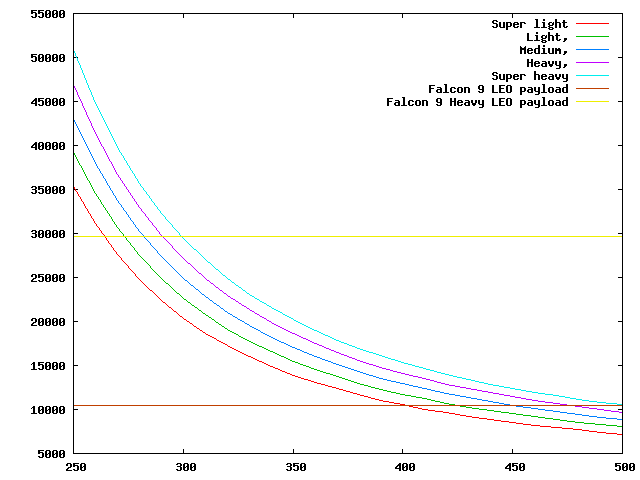
\includegraphics[scale=0.6]{images/fuel_analysis}
\caption{Total launch mass of CLLARE lunar landing mission configuration for various specific impulses.}
\end{figure}

Figure \ref{fig:fuel_analysis} shows the total launch mass (i.e. vehicles and fuel) for a lunar landing configuration of the core hardware versus various specific impulses, for a variety of vehicle mass estimates.  The ``baseline'' mass estimate, the case labelled ``Medium'' in the plot, has the values shown in Table \ref{tab:fuel_analysis} below.  The cases labelled ``Heavy'' and ``Super heavy'' have all values except the astronaut mass increased by 10\% and 20\% respectively, while the cases labelled ``Light'' and ``Super light'' have all values except the astronaut mass decreased by 10\% and 20\% respectively.  The delta-v requirements used to generate the plot are those listed in Table \ref{tab:deltav-budget} below, with a 10\% additional allowance for each burn as a ``safety margin'' to allow for occasional corrections.  Horizontal lines on the plot show the maximum LEO payloads of the Falcon 9 and Falcon 9 Heavy launch vehicles.

\begin{table}
\centering
\caption{``Medium'' mass estimates for lunar landing configuration.}
 \label{tab:fuel_analysis}
\begin{tabular}{ | l | c | }
\hline
\textbf{Hardware item} & \textbf{Mass} \\
\hline
\hline
CM		& 1008 kg \\
\hline
Astronaut	& 75 kg \\
\hline
EVA suit	& 100 kg \\
\hline
OSM		& 200 kg \\
\hline
LL		& 300 kg \\
\hline
PM		& 500 kg \\
\hline
\end{tabular}
\end{table}

\begin{table}
\centering
\caption{Delta-v budget for lunar landing flight.}
\label{tab:deltav-budget}
\begin{tabular}{ | l | c | }
\hline
\textbf{Burn} & \textbf{Delta-v} \\
\hline
\hline
TLI	& 3276 m/s \\
\hline
LOI	& 1000 m/s \\
\hline
Lunar ascent/descent	& 4700 m/s \\
\hline
TEI	& 700 m/s \\
\hline
\end{tabular}
\end{table}

Using the ``Medium'' mass estimates, the figure shows that if the Falcon 9 is to remain viable as a launch vehicle, a specific impulse of around 450s will be required.  This is at the far upper end of impulses achievable using LOX/LH2, making that the only feasible choice of propellant for a hardware configuration of this mass.

Note that the ``Heavy'' mass estimate, which adds just 10\% to the ``Medium'' estimate, requires a specific impulse of around 475 s.  This is unrealistic using LOX/LH2 or any other propellant combination CSTART is aware of, suggesting that current mass estimates are right on the line of feasibility and great care must be taken to ensure the actual hardware masses do not exceed the ``Medium'' estimates.

Note that for LOX/LCH4 to be a feasible propellant, the ``Medium'' estimate would need to turn out to be excessive by more than 20\% -- probably somewhere around 30\%.  This unlikely, although not impossible.

In light of the results of this analysis, which suggest that the common PM/LL engine may need a specific impulse of 450s, we use the lower end point of the fuelled mass range for circumlunar flights found in the previous section, i.e. 3679 kg.
\subsection{Total launch masses}

The table below summarises estimated total launch masses for various configurations of the CLLARE core hardware, using the estimates developed in the preceeding sections of this chapter.

\begin{tabular}{ | l | c | }
\hline
Configuration & Estimated total mass (kg) \\
\hline
\hline
Suborbital (CM) & 1000 \\
\hline
Short Orbital (CM-OSM without consumables) & 1250 \\
\hline
Long Orbital (CM-OSM with consumables) & 1350 \\
\hline
High Altitude Orbital, Circumlunar & 3679 \\
(CM-OSM-PML) & \\
\hline
Lunar Landing (CM-OSM-LLH-PMH) & 10,000 \\
\hline
\end{tabular}

\section{Cost figures}

\subsection{Vehicle costs}

\subsection{Fuel costs}

\subsection{Launch costs}

By far the greatest contributing factor to total flight costs will be the cost of launch to LEO. 

\subsubsection{Suborbital and orbital missions}

Unknown (self-built modular hybrid booster)

\subsubsection{Circumlunar missions}

\subsubsection{Lunar landing missions}

A single launch of the Falcon 9 commercial booster costs US\$35,000,000.

\subsection{Total costs}

%%%%%%%%%%%%%%%%%%%%%%%%%%%%%%%%%%%%%%%%%%%%%%%%%%

\chapter{Detailed Hardware Descriptions} \label{chap:detail}

In this chapter we present detailed descriptions of some of the CLLARE core hardware items.  Complete technical descriptions and diagrams of all hardware items will be compiled into a separate publication at a future time.

\section{The CLLARE Command Module}

\subsection{Overview}

\begin{itemize}
\item Reusable
\item Glass cockpit
\item Lifting reentry
\item Paraglider landing
\end{itemize}

\subsection{Structure and construction}

\begin{figure}[ht] \label{fig:cm_structure}
\centering
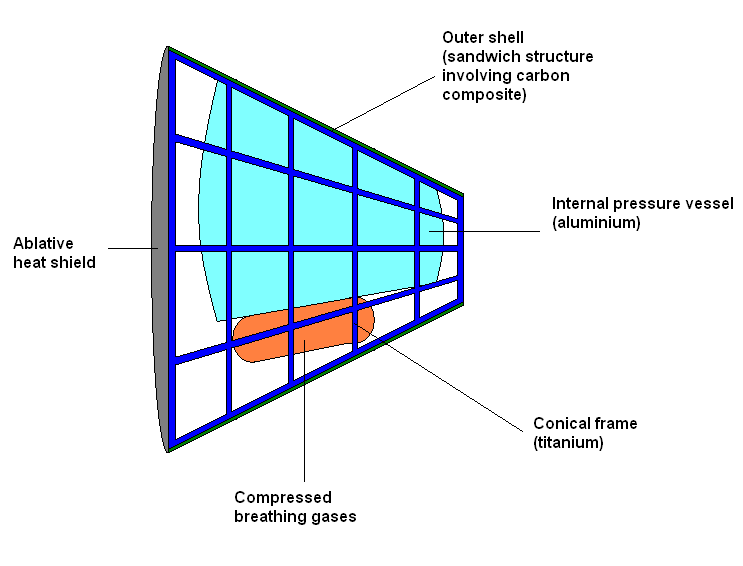
\includegraphics[scale=0.6]{images/cllare_cm_structure_concept}
\caption{Concept diagram for main structure of CLLARE Command Module.  Diagram not to scale.}
\end{figure}

\begin{figure}[ht] \label{fig:cm_internals}
\centering
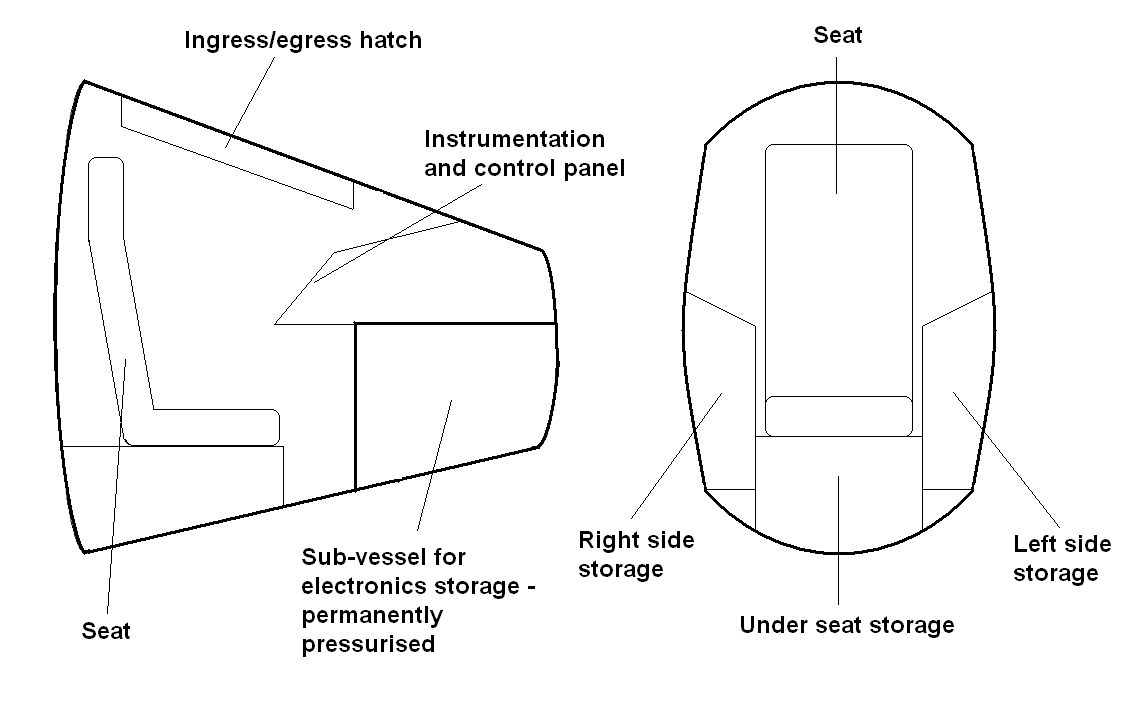
\includegraphics[scale=0.3]{images/cllare_cm_pressure_vessel_contents}
\caption{Concept diagram for contents of CLLARE Command Module pressure vessel.  Diagram not to scale.}
\end{figure}

The proposed structure of the conical part of command module (picutred in Figure \ref{fig:cm_structure} consists of a conical frame built from titanium, with an ablative heat shield acting as a base cap and an outer shell covering the rest of the frame, providing heat shielding during reentry and insualtion while in space.  Inside of the frame is mounted an aluminium pressure vessel with an ingress/egress hatch on the top, featuring a window.  The heat shield and the shell are necessarily single--use only.  The pressure vessel and its contents are intended be reusable.  The reusability of the frame will be determined later after consideration of the forces it may be subject to during a flight.

The pressure vessel (pictured in Figure \ref{fig:cm_internals}) is divided into two separate parts.  The largest part of the pressure vessel is where the astronaut is seated during flight.  This part of the pressure vessel is vented prior to EVA, so everything inside it must be vacuum safe.  A second, much smaller pressure vessel in the front and bottom of the main vessel contains the air--breathing fuel cells and all electronics.  This pressure vessel remains pressurised at all times, including during EVA, facilitating the use of commercial Earth--based electronics.  While the main part of the vessel is pressurised, the flow of gas between the two pressure vessels is permitted by open valves, so that heat generated by the electronics is able to heat the cabin.  Injection of oxygen into the pressure vessel happens through the smaller vessel, so that the fuel cells can continue to run while EVA is in progress.

TODO: Need to discuss structure of nose cylinder.

\subsection{Reaction Control System}

The \href{http://cstart.org/wiki/CLLARE_CM_Reaction_Control_System}{CM's Reaction Control System} (RCS) provides pitch, yaw and roll control for the CM, to be used both during spaceflight and reentry. It is the CM's only self-contained means of propulsion.

An RCS based on the use of cold gas such as nitrogen or carbon dioxide would be preferred for simplicity and safety, but there are concerns about the performance of such systems being able to meet the necessary demands.  If cold gas cannot be made to work, the use of hydrogen peroxide monopropellant rockets may be considered preferentially to full blown bipropellant liquid rockets.

\subsection{Power system}

The \href{http://cstart.org/wiki/CLLARE_CM_Power_System}{CM's power system} provides 12V and 24V DC power to other subsystems, generated by an array of small and rugged atmosphere breathing methanol fuel cells, such as the \href{http://www.ultracellpower.com/assets/XX55_Data_Sheet_01-27-2009.pdf}{Ultracell XX55}.  A set of backup batteries provide continuity of power during temporary interruptions to methanol or oxygen supplies.

\begin{tabular}{ | l | c | c | c | c | }
\hline
Application & Voltage & Unit Power & Multiplier & Total power \\
\hline
\hline
USRP comms board & 6V & ?? & 1 & ?? \\
\hline
Crossbow NAV440 & 9-42 & $<4$ W & 1 & $<4$ W \\
GPS/IMU unit & & & & \\
\hline
\hline
Total power requirement & & & & $<4$ W \\
\hline
\end{tabular}

\subsection{Environmental Control System}

The \href{http://cstart.org/wiki/CLLARE_Environmental_Control_System}{CM's Enviromental Control System} is responsible for maintaining a habitable environment inside the CLLARE Command Module cabin. This involves maintaining an appropriate oxygen, pressure and humidity levels, temperature and more.

Little design work on the ECS has been performed thus far.  The use of a 20\% oxygen, 80\% nitrogen atmosphere maintained at room temperature is considered attractive as it enables the use of commercial electronics without modification.

\subsection{Waste Management System}

The \href{http://cstart.org/wiki/CLLARE_Waste_Management_System}{CM's Waste Management System} is responsible for the collection and storage of bodily waste for the duration of flights.

Little design work on the WMS has been performed thus far, though we are keen to improve on the much--hated ``Apollo bags'' of previous lunar missions, to the extent that we can within our space and mass restrictions.  The Soyuz/Mir space toilet is a possible source of inspiration.

\subsection{Communication System}

The \href{http://cstart.org/wiki/CLLARE_CM_Communication_System}{CM's Communication System} provides the means for communication between the CM and Earth and the Lander and Earth (the Lander's comm system uses the CM's system as a relay).

There are four communication channels required between the CM and Earth:
\begin{itemize}
\item A bidirectional voice link (VO),
\item A unidirectional, space-to-Earth video downlink (VI),
\item A unidirectional, space-to-Earth telemetry downlink (TM), and
\item A unidirectional, Earth-to-space telecommand uplink (TC).
\end{itemize}
We hope to realise these four channels as independent ``virtual channels'' on a single physical channel, using a multiplexing technology such as \href{http://en.wikipedia.org/wiki/Code_division_multiple_access}{Code Division Multiple Access} (CDMA).

The single physical channel linking the CM to Earth will likely be an S-band radio link in the 2.0 GHz -- 2.4 GHz range, depending on which frequencies are available for use in the various parts of the world where we may operate communication systems.

The use of \href{http://en.wikipedia.org/wiki/Software_defined_radio}{software-defined radio} (SDR) technology for the communications system is considered an attractive option due to its reduced equipment mass and high flexibility.  The \href{http://gnuradio.org/redmine/wiki/gnuradio}{GNU Radio project} and the \href{http://www.ettus.com/products}{Universal Software Radio Peripheral (USRP) device} provide open source software and hardware, respectively, which may help to realise the SDR approach at a very low cost.  However, no hard decision has been made and investigations are ongoing.

\subsection{Navigation System}

The \href{http://cstart.org/wiki/CLLARE_CM_Navigation_System}{CM's Navigation System} uses various hardware sensors and interactions with other subsystems to provide high accuracy estimates of position, orientation and translational and rotational velocities at all stages of the mission.  Plans for the navigation system include the use of GPS, inertial measurement units, radio round--trip--time and Doppler shift measuremets, StarTrackers and more.

The integration of data from this varied range of sources, each with distinct inherrent accuracies and error profiles, into a single, optimal estimate of position, orientation and velocities will require the use of ``filtering'' software, such as Kalman filters or recursive Bayesian estimation.

\subsection{Computer System}

The \href{http://cstart.org/wiki/CLLARE_Main_Computer_System}{CM's Main Computer System} provides computational services for most other subsystems, including but not limited to:
\begin{itemize}
\item Encoding of audio and video data for onboard storage and transmission by the communications system.
\item High--reliability onboard storage of audio, video, telementry and navigation data.
\item Control of oxygen injection valves for the environmental control system.
\item Kalman filtering for the navigation system.
\item Formatting of raw sensor data into telemetry packets for the communicaton system.
\item Authentication and execution of telecommands for the communicaton system.
\end{itemize}

\subsubsection{Hardware}

The issue of radiation shielding for space--fairing computers is of considerable importance.  Special radiation--hardened CPUs for us in space exist, but these are both difficult to acquire and significantly underpowered compared to the leading edge of consumer computer hardware.  Thus we expect that the CLLARE Main Computer System will use consumer computer hardware which will be protected from radiation by custom--built shielding.  The desire to minimise the mass of this shielding provides a strong motivation for keeping the computer hardware as compact as possible.  It is anticipated that small, cheap, low-power embedded systems like (but not necessarily) the \href{http://beagleboard.org}{BeagleBoard} will best meet our requirements.

\subsubsection{Software}

The CSTART Social Contract stipulates that ``all computers onboard CSTART rockets and spacecraft which run operating systems will run operating systems whose kernel and basic userland utilities satisfy the Free Software Foundation's Free Software Definition''.  Thus, it is likely that a GNU/Linux distribution or one of the free BSD--derived operating systems will be used.  The userland software running on this operating system will necessarily have to be custom developed by CSTART volunteers.  The Social Contract stipulates that this software will be GPL3 licensed, and development is expected to happen in an open and decentralised fashion.

\section{The CLLARE Orbital Support Module}

Discuss rocket options here.

Discuss required consumables and storage options here: oxygen, nitrogen, methanol, water, anything else?

%%%%%%%%%%%%%%%%%%%%%%%%%%%%%%%%%%%%%%%%%%%%%%%%%%

\section{The CLLARE Propulsion Module}

\begin{figure}[h] \label{fig:pm}
\centering
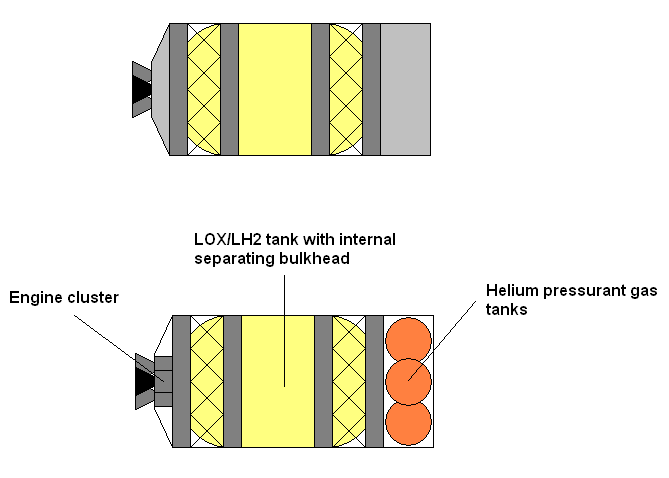
\includegraphics[scale=0.6]{images/cllare_pm_concept}
\caption{Concept diagram for CLLARE Propulsion Module, with external view (top) and internal view (bottom).  Diagrams not to scale.}
\end{figure}

\subsection{Propellant tank}

Both the fuel and oxidiser for these rockets are stored in the one tank, with an internal bulkhead providing separation and insulation of the two propellants.  Helium gas is used as a pressurant to force the propellants into the combustion chambers.

\subsection{Engines}

The PM features an ``engine cluster'' at its rear, consisting of a symmetric arrangement of 4 or 5 engines in a ``cross shape''.  These engines are precisely the same as the engine used on the Lunar Lander.  The cross shaped cluster of engines permits some degree of steering of hardware configurations using the PM, via differential thrusting of various engines.  Failure of individual engines can be compensated for by shutting down the opposite engine (obviously not required in the case of the central engine in a 5 engine cluster).

In Section \ref{sec:ll_engine} we calculate that the Lunar Lander's engine will need to provide at least a thrust of 3.5 kN for lunar descent/ascent.  Thus a cluster of 4 or 5 of these engines will provide a total PM thrust of between 14 and 17.5 kN (compared with 91.2 kN for the Apollo Service Module's engine).  With a fully fuelled mass of around 10,000 kg, this leads to an initial acceleration during TLI of between 1.4 and 1.75 m/s/s.  This is a very low acceleration compared to Apollo TLI (which peaked at around 1.5 g or just under 15 m/s/s), which will necessitate a longer duration TLI burn.

%%%%%%%%%%%%%%%%%%%%%%%%%%%%%%%%%%%%%%%%%%%%%%%%%%

\section{The CLLARE Lunar Lander}

\begin{figure}[h] \label{fig:ll}
\centering
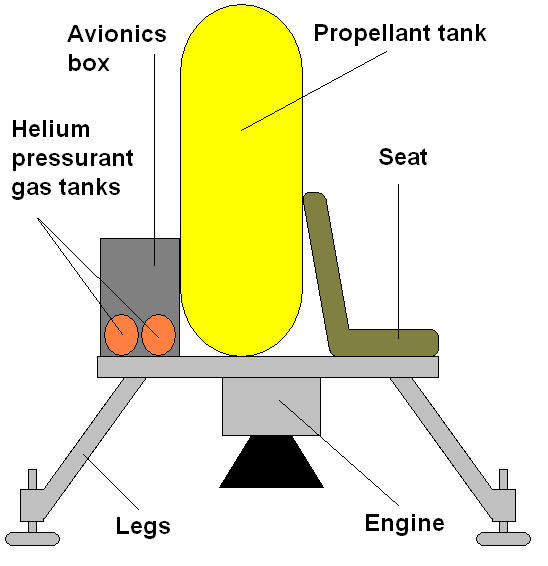
\includegraphics[scale=0.6]{images/cllare_ll_concept_labelled}
\caption{Concept diagram for CLLARE Lunar Lander.  Diagrams not to scale.}
\end{figure}

\subsection{Overview}

The CLLARE Lunar Lander is an extremely minimalist lunar landing vehicle, inspired by a wide range of minimalist landing plans from the Apollo era.  Its most striking difference compared to the Apollo Lunar Module is the fact that it is an ``open cab'' design: the astronaut is not enclosed inside a pressure vessel of any kind.  Instead the astronaut is seated in a seat attached to the exterior of the lander, wit life support provided by the EVA suit.  Harness and restraint technology from moder roller coasters and similar amusement rides are expected to be a source of inspiration for making this arrangement as safe as possible.  Unlike the Apollo LM, the CLLARE LL is a single stage vehicle, using the same engine and fuel tanks to power both descent and ascent.  The CLLARE LL has three legs arranged in an equilateral triangle configuration, rather than four legs in a square configuration, in order to minimise mass.  It is hoped that modern computers and navigation electronics will facilitate an almost completely automated descent process for the LL.

\subsection{Reaction Control System}

As with the Command Module, an RCS based on the use of cold gas such as nitrogen or carbon dioxide would be preferred for simplicity and safety.  Note that the LL's RCS must be capable of controlling orientation and position independently.  A set of four ``thruster blocks'', mounted symmetrically in a cross shape, with each thruster block containing 4 orthogonal thrusters, is probably the most straightforward way to achieve this.

\subsection{Power system}

Long life batteries are probably the most realistic choice of power source for the lander, since its operational life time will be too short for fuel cells to be worth while.

\subsection{Communication System}

The communications system of the LL will be similar to that of the CM in many respects (such as the use of software-defined radio and multiplexing technology).  However, there will be no telecommand channel (the delay in radio communication between the Earth and moon will prevent the reliable piloting of the LL by remote control from Earth).  The LL is expected to use the orbiting CM as a communications relay rather than transmitting directly to Earth itself.  This will result in radio black outs while the CM is behind the moon from the LL's point of view, but the alternative is to drastically increase the transmission power and antenna size of the LL's communication system, resulting in a higher power demand and a more massive lander.

\subsection{Navigation System}

The main difference between the LL's navigation system and the CM's is that the LL will require an altimeter of some kind.  An Australian--New Zealand group called \href{http://www.lunarnumbat.org}{Lunar Numbat} are working on (amongst other things) an \href{http://www.lunarnumbat.org/cgi-bin/twiki/view/LunarNumbat/LNTaskRadarAltimeter}{open source radar altimeter} for use by one of the Google Lunar X Prize teams, which may be appropriate.

\subsection{Engine} \label{sec:ll_engine}

We put an initial estimate on the required thrust of the LL engine, despite not having a careful descent plan, by using figures from the Apollo Lunar Module.  The Apollo LM's descent stage mass was 10,149 kg and the ascent stage mass was 4,547 kg, for a total LM mass of 14,696 kg.  The LM's descent engine produced a thrust of 44.40 kN, resulting in a descent acceleration of 3.02 m/s/s.  The LM's ascent engine produced a thrust of 15.6 kN, resulting in an ascent acceleration of 3.43 m/s/s.  We estimate the fuelled mass of the CLLARE LL to be no greater than 1000 kg.  Thus to produce an acceleration of up to 3.5 m/s/s, to roughly match maximum Apollo acceleration, requires an engine thrust of 3.5 kN. 

It has not yet been determined whether or not the LL engine will be gimballed or whether it will be fixed, with orientation of the LL via RCS taking the place of gimballing.

\subsection{The CLLARE Lunar EVA Suit}

Someone needs to expand on this:
\begin{itemize}
\item Needs to be suitable for EVA in LEO, in lunar orbit, on lunar surface.
\item Needs to support a few hours of activity without external supplies.
\item Needs to be as light as possible.
\item Elasticated, mechanical counter--pressure concept (Webb et. al.) looks promising.
\item Will work closely with Open Luna Foundation.
\end{itemize}

\chapter{Concept Art}

This chapter contains various items of concept art for the CLLARE project.

In many items of concept art, items of the CLLARE core hardware are depicted bearing a flag which features an image of the Earth from space on a blue background.  The reason for this is that CSTART is an official partner of the \href{http://www.oneflaginspace.org}{One Flag in Space} project, whose mission is ``to promote the use of the ``Blue Marble'' as a symbol of world unity in space exploration. It is a symbol that anyone, anywhere in the world can relate to, regardless of nationality, ethnic origin or religious beliefs, yet does not require political collaboration between space-faring nations''.  The CSTART Social Contract stipulates that, in support of the ideals of One Flag in Space, all CSTART spacecraft shall bear the Blue Marble flag, and that no CSTART spacecraft shall bear the flag of any nation of Earth.

\begin{figure}[h] \label{fig:cm_on_modular_booster}
\centering
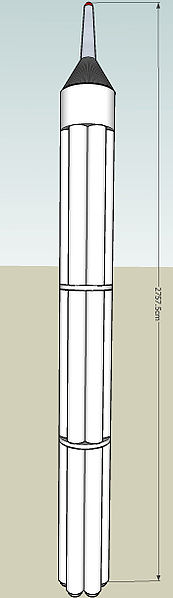
\includegraphics[scale=0.6]{images/cm_on_modular_booster}
\caption{Concept rendering of CLLARE Command Module atop a booster made of simple, modular hybrid rockets.  Render not to scale.}
\end{figure}

\begin{figure}[h] \label{fig:cllare_lunar_landing_config}
\centering
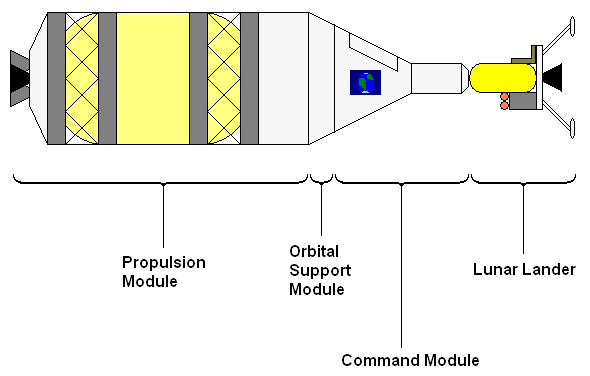
\includegraphics[scale=0.6]{images/cllare_lunar_landing_config}
\caption{Concept diagram for lunar landing configuration of CLLARE core hardware.  Diagram not to scale.}

\end{figure}
\end{document}
